%%%%%%%%%%%%%%%%%%%%%%%%%%%%%%%%%%%%%%%%%%%%%%%%%%%%%%%%%%%%%%%%%%%%%%%%%%%%%%%%%%%%%%%%%%%%%%%%%%%
%%%%%%%%%%%%%%%%%%%%%%%%%%%%%%%%%%%%%%%%%%%%%%%%%%%%%%%%%%%%%%%%%%%%%%%%%%%%%%%%%%%%%%%%%%%%%%%%%%%

\section{Conceptos, matem\'aticas}

En esta secci\'on se describen los conceptos b\'asicos de la teor\'ia espectral 'cl\'asica' para 
procesos estacionarios, y la generalizaci\'on hecha por Priestley para procesos no-estacionarios. 
De forma m\'as bien pragm\'atica, la descripci\'on est\'a
 fuertemente inspirada por el libro 'Spectral Analysis and Time Series' 
de M. B. Priestley \cite{Priestley81}, ya que este est\'a expl\'icitamente dirigido a un p\'ublico 
sin un trasfondo matem\'atico.

Se suponen conocidos varios temas b\'asicos de probabilidad y estad\'istica:
variables aleatorias, valores esperados y momentos, estimadores y sus propiedades.
Con el fin de presentar la notaci\'on usada, se incluyen algunos conceptos previos a la 
definici\'on per se de estacionariedad y estimadores en el dominio de frecuencias.
%Chatfield (The Analysis of Time Series: An Introduction, 2003)

%%%%%%%%%%%%%%%%%%%%%%%%%%%%%%%%%%%%%%%%%%%%%%%%%%%%%%%%%%%%%%%%%%%%%%%%%%%%%%%%%%%%%%%%%%%%%%%%%%%

\subsection{Estacionariedad d\'ebil}

Para hablar formalmente de procesos estoc\'asticos como modelos, antes 
conviene escribir su definici\'on desde el punto de vista matem\'atico. Las siguientes definiciones
son aplicables tanto para procesos en tiempo continuo
como para procesos a tiempo discreto; aunque el objeto de estudio, el EEG, se considera 
un fen\'omeno continuo, s\'olo es posible registrarlo durante un conjunto finito de puntos 
en el tiempo.

\begin{defn}[Proceso estoc\'astico]
Un proceso estoc\'astico $\{ X(t) \}$ es una familia de variables aleatorias 
en los reales,
indexadas por
$t \in T \subseteq \R$.
%, mientras que una observaci\'on
%de $\{X(t)\}$ ser\'a denotada por $(x_1,x_2,\dots)$
\end{defn}

Como notaci\'on, una realizaci\'on de $X(t)$ ser\'a denota por $x_t$. 
Las funciones de densidad de probabilidad y de probabilidad acumulada para $X(t)$ ser\'an
referidas, respectivamente, como $f_{X(t)}$ y $F_{X(t)}$
%Cabe destacar que en esta definici\'on se omiti\'o intencionalmente pedir que las variables
%aleatorias sea reales, ya que eventualmente se considerar\'an procesos en los complejos.
Cabe enfatizar que para cada valor de $t$,
%tiempo $t$, 
$X(t)$ es una variable aleatoria; no se presupone ninguna conexi\'on entre ellas.
%con su funci\'on de densidad de probabilidad,
%sus momentos [s\'olo se consideran va's con al menos segundos momentos finitos], etc.


La caracter\'istica principal 
investigada en este trabajo hace referencia a la ''estacionariedad''. De manera 
informal, esta propiedad se refiere a que las variables aleatorias que conforman un proceso
estoc\'astico sean b\'asicamente iguales --dicho con otras palabras, que las propiedades
del proceso sean invariantes en el tiempo. 
Una definici\'on que satisface fielmente est\'a descripci\'on es la de estacionariedad 
en el sentido fuerte o estricto.
El t\'ermino ''tiempos admisibles'' simplemente indica que la definici\'on es la misma para
procesos a tiempo discreto o continuo, bajo restricciones obvias.

\begin{defn}[Estacionariedad fuerte]
Un proceso estoc\'astico $\{ X(t) \}$ es fuertemente estacionario si, para cualquier 
conjunto de tiempos admisibles $t_1,t_2,\dots,t_n$ y cualquier $\tau$ tal que 
 $t_i+\tau$ son tiempos admisibles para $i = 1, 2, \dots n$;
se cumple que
\begin{equation*}
F_{\left(X(t_1),X(t_2),\dots,X(t_n)\right) }
\equiv
F_{\left(X(t_1+\tau),X(t_2+\tau),\dots,X(t_n+\tau)\right)}
\end{equation*}

Donde $F_{\left(X(t_1),X(t_2),\dots,X(t_n)\right) }$ es la funci\'on de distribuci\'on de
probabilidad conjunta del vector $\left(X(t_1),X(t_2),\dots,X(t_n)\right)$
\end{defn}

Esta definici\'on, sin embargo, no resulta muy \'util en el contexto de la estad\'istica:
si se supone que el registro de un fen\'omeno puede interpretarse como \textbf{una} 
realizaci\'on de
un proceso estoc\'astico, entonces para cada tiempo se tiene una \'unica observaci\'on
de cada variable aleatoria. A esto hay que a\~nadir que, para un fen\'omeno continuo,
no todas los tiempos son registrables.
Luego, si no existe la garant\'ia de que las propiedades de estas variables aletorias sean
''similares'', entonces es virtualmente imposible obtener mayor informaci\'on de ellas.

Es bajo estas limitaciones que se motiva un concepto de estacionariedad m\'as d\'ebil, pero que
satisfaga ''suficientes teoremas importantes'' y que sea relevante bajo las restricciones
propias de diferentes campos. En este trabajo se ha optado por la llamada 
''estacionariedad d\'ebil'' o estacionariedad de orden 2, que recibe su nombre como caso
particular de la ''estacionariedad de orden $m$''.

\begin{defn}[Estacionariedad de orden $m$]
Un proceso estoc\'astico $\{ X(t) \}$
se dice estacionario de orden $m$ si, para cualquier 
conjunto de tiempos admisibles $t_1,t_2,\dots,t_n$ y cualquier $\tau \in \R$
se cumple que
\begin{equation*}
\E{ X^{m_1}(t_1)X^{m_2}(t_2)\cdots X^{m_n}(t_n) }
=
\E{ X^{m_1}(t_1+\tau)X^{m_2}(t_2+\tau)\cdots X^{m_n}(t_n+\tau) }
\end{equation*}
Para cualesquiera enteros $m_1,m_2,\dots,m_n$ tales que $m_1+m_2+\dots+m_n \leq m$
\label{est_orden_m}
\end{defn}

La estacionariedad d\'ebil no pide que la funci\'on
de distribuci\'on conjunta tenga determinada forma, sino que los momentos conjuntos sean 
invariantes ante traslaciones en el tiempo. Para entender mejor esta diferencia, consid\'erense
tres procesos $\{X(t)\}$, $\{Y_1(t)\}$ y $\{Y_2(t)\}$, de modo que el primero es
estacionario en el sentido fuerte, el segundo es estacionario de orden 1 y el tercero es
estacionario de orden 2.
\begin{itemize}
\item Por definici\'on $F_{X(t) } \equiv F_{X(t+\tau)}$ para cualesquieras $t$, $t+\tau$
admisibles; entonces $\E{X(t)} = \mu_X$ es constante
\item Por definici\'on
para cualesquieras $t$, $t+\tau$ admisibles se tiene que $\E{Y_1(t)}=\E{Y_1(t+\tau)}$ y
$\E{Y_2(t)}=\E{Y_2(t+\tau)}$. Se deduce que $\E{Y_1(t)} = \mu_{Y_1}$, 
$\E{Y_2(t)} = \mu_{Y_2}$ son constantes
\item Usando nuevamente que $F_{X(t) } \equiv F_{X(t+\tau)}$ para cualesquieras $t$, $t+\tau$
admisibles, se deduce que $\Var{X(t)} = \sigma_X$ es constante
\item Por definici\'on de $\mathrm{Var}$ y de $Y_i$ ($i=2,1$)
$$\Var{Y_i(t)} = \E{Y_i^{2}(t)} - \left( \E{Y_i(t)} \right)^{2} = \E{Y_i^{2}(t)} - \mu_{Y_i}$$
Luego se puede deducir que 
$\Var{Y_2(t)}$ es
% $\E{Y_2^{2}(t)}$ es
constante, mientras que no se puede garantizar lo mismo para $\Var{Y_1(t)}$
% Se concluye que la varianza
%de $Y_2$ es constante en el tiempo mientras que la de $Y_1$ no necesariamente lo es
\item El \textit{coeficiente de asimetr\'ia de Fisher} 
de una variable aleatoria $V$ se define como
$$
\gamma_1(V) = \frac{\E{\left(V-\E{V}\right)^{3}}}{\Var{V}^{\nicefrac{3}{2}}}
$$
%= \frac{\E{X^{3}}-3\mu_V \E{V^{2}}+2\mu_V^{3}}{\Var{V}^{\nicefrac{3}{2}}}
%$$
Sin entrar en detalles, se puede deducir que $\gamma_1(X(t))$ es constante mientras que no se
puede garantizar lo mismo para $\gamma_1(Y_1(t))$, $\gamma_1(Y_2(t))$
\end{itemize}

Naturalmente hay una relaci\'on de contenci\'on clara en
la familia de los conjuntos de procesos estacionarios de orden finito:
si un proceso es estacionario de orden $m$, entonces es estacionario de orden $n$ para todo
$n \leq m$. Es posible incluso describir procesos que sean estacionarios de orden ''infinito''
y preguntarse bajo qu\'e condiciones son fuertemente estacionarios.
Tal discusi\'on no se incluye en el presente trabajo.
%,
%% con el fin de ser concreto.
%ya que 
%%el enfoque es de modelaci\'on y 
%se ha intentado hacer la menor cantidad posible de supuestos y de proporcionara a cada uno una
%''interpretaci\'on fisiol\'ogica''.


%As\'i pues, y dadas 
Una vez hechas
las consideraciones anteriores, conviente
introducir una segunda caracter\'izaci\'on de los procesos estacionarios de orden 2 --d\'ebilmente 
estacionarios--
% enlistar las siguientes propiedades para un proceso
%estacionario de orden 2 --o d\'ebilmente estacionario-- 
que es equivalente
%\footnote{Este hecho se vuelve claro si se analizan cuidadosamente las propiedades
%enlistadas y se comparan con las deficiniones de las ''cantidades'' involucradas}
a la definici\'on \ref{est_orden_m} pero cuya interpretaci\'on suele considerarse como m\'as clara
%Hay una especie de consenso seg\'un el cual la estacionariedad de orden 2, tambi\'en
%llamada \textbf{estacionariedad d\'ebil} es suficiente para
%que se cumplan los teoremas m\'as comunes sobre medias y varianzas.
%Algunas consecuencias que un
%proceso sea estacionario debilmente son las siguientes:
\begin{thrm}
Un proceso es d\'ebilmente estacionario si y s\'olo si para cualesquiera tiempos admisibles
$t$, $s$ se tiene que
\begin{itemize}
\item $\E{X(t)} = \mu_X$
\item $\Var{X(t)} = \sigma^{2}_X$
\item $\Cov{X(t),X(s)} = \rho (s-t)$
\end{itemize}
Donde $\mu_X$, $\sigma^{2}_X$ son constantes, $\rho(\tau)$
es una funci\'on que \'unicamente depende de $\tau$
\label{est_usual}
\end{thrm}

A grosso modo, cuando uno se refiere a un proceso d\'ebilmente estacionario seg\'un
\ref{est_orden_m} se le pide que su primer y segundo momentos sean constantes, as\'i como
el primer momento conjunto s\'olo dependa del lag en el tiempo. A su vez, seg\'un 
\ref{est_usual} un proceso es d\'ebilmente estacionario si su media y varianza son constantes en
el tiempo, y su funci\'on de autocovarianza s\'olo depende del lag en el tiempo.

Cabe mencionar, como comentario, que es posible contruir procesos que sean fuertemente
estacionarios pero que no sean estacionarios de ning\'un orden finito; dado que
la primera definici\'on se basa en funciones de densidad de probabilidad mientras que la segunda
se basa en momentos, es suficiente con usar variables aleatorias que no tengan todos
sus momentos bien definidos. Por ejemplo, consid\'erese un proceso conformado por variables
aleatorias independientes id\'enticamente distribuidas con distribuci\'on de Cauchy.

Dado que en el EEG se miden fluctuaciones en potenciales de campos el\'ectricos
%(medida en mV),
que (en este trabajo) se modelan como variables aleatorias, 
la intepretaci\'on usual para los momentos de estas variables est\'a ligado a la distribuci\'on de
energ\'ia asociada al sistema. Luego, es plausible considerar que el EEG es un fen\'omeno
''suficientemente regular'' como para que las variables aleatorias del modelo tengan cuando
menos segundos momentos bien definidos.

%%%%%%%%%%%%%%%%%%%%%%%%%%%%%%%%%%%%%%%%%%%%%%%%%%%%%%%%%%%%%%%%%%%%%%%%%%%%%%%%%%%%%%%%%%%%%%%%%%%

\subsection{Espectro de un proceso estacionario}

Existe una larga tradici\'on en las ciencias biom\'edicas para interpretar a los registros
electrofisiol\'ogicos en t\'erminos de ondas y frecuencias, ya que fundamentalmente se
trata de fen\'omenos el\'ectricos \cite{Kaiser00}. 
As\'imismo existe una teor\'ia matem\'atica bien desarrollada sobre estad\'istica en el 
llamado ''dominio de las frecuencias''. 
En este trabajo se aborda la segunda como forma de tener coherencia con la primera; a continuaci\'on
se describen los conceptos m\'as importantes en el modelo usado.

Un objeto fundamental para el estudio del dominio de las frecuencias\footnote{Este concepto 
no se
%discutir\'a en el presente trabajo, sino que 
ser\'a manejado pragm\'aticamente para referirse
al cambio de coordenadas inducido por la transformada de Fourier o alguna generalizaci\'on de la 
misma} son las series de Fourier y sus generalizaciones. 

\begin{defn}[Serie de Fourier]
Sea $f$ una funci\'on peri\'odica con periodo $2\pi$ tal que $\intR \abso{f(t)} dt < \infty$. 
Si se calculan los coeficientes
\begin{equation*}
A_n = \frac{1}{2\pi} \intPI f(t) e^{- i n t} dt
\end{equation*}
entonces la siguiente igualdad se cumple casi en todas partes
\begin{equation*}
f(x) = \sum_{n=-\infty}^{\infty} A_n e^{i n t}
\end{equation*}
La sucesi\'on $\left( A_n \right)$ ser\'a referida como \textbf{serie de Fourier} de la funci\'on
$f$.
\label{FourierClasico}
\end{defn}

%\begin{defn}[Transformada de Fourier (funciones peri\'odicas)]
%Sea $f$ una funci\'on peri\'odica con periodo $2\pi$ tal que $\intR \abso{f(t)} dt < \infty$.
%hjkjkjkj
%\end{defn}

Por el momento no se discutir\'an los detalles sobre la convergencia de las sucesiones de 
\ref{FourierClasico}, siempre que se limite a funciones 
peri\'odicas,
continuas y absolutamente sumables,
%$L^{1}\left([-\pi,\pi])\right)$
o se permita que sean acotadas y con
una cantidad finita de discontinuidades --y se ponga ninguna atenci\'on sobre ellas.
Parece claro que se puede definir una funci\'on --quiz\'a invertible-- que mapee funciones 
a sus respectivas series de Fourier;
%que
%poseen serie de Fourier a ''alg\'un'' conjunto de series absolutamente sumables $\ell$; 
esta
funci\'on es referida como \textbf{transformada de Fourier}. Por lo pronto se considerar\'a
que las propiedades y limitaciones de la transformada de Fourier son conocidas
al menos a grosso modo, m\'as que nada por brevedad; se pretende exhibir
el espectro de potencias para una serie de tiempo como una extensi\'on de la
transformada de Fourier de modo que se espera
poder enfatizar sobre algunas
interpretaciones dentro de la modelaci\'on.
%conocidas y demostradas todas sus propiedades.

%%%%%%%%%%%%%%%%%%%%%%%%%%%%%%%%%%%%%

\subsubsection{Notas sobre interpretaci\'on f\'isica}

Las series de Fourier gozan de una interpretación física muy extendida como que una 
se\~nal\footnote{Esta palabra se usar\'a para referirse a un fen\'omeno f\'isisco 
que est\'a siendo 
registrado, bajo el entendido que es casi lo mismo referirse al registro o al proceso
que lo genera si \'este es determinista}
peri\'odica
puede verse como la superposici\'on de se\~nales peri\'odicas m\'as simples. 
De igual forma es destacable su interpretaci\'on como ''coordenadas'' en un espacio de funciones
dada una base ortonormal del mismo. 
El estudio de estos espacios dentro del an\'alisis trae a la mente
la cuesti\'on de convergencia,
el problema del subespacio de
funciones medibles de medida cero, y la posibilidad de otras bases; estos fen\'omenos tienen a su 
vez una interpretaci\'on f\'isica como cambios s\'ubitos en la energ\'ia, el ruido y la 
tipificaci\'on de ondas ''simples'' --por ejemplo, las ondas cuadradas y triangulares son 
m\'as comunes en teor\'ia de circuitos.

Para limar estas ambig\"uedades, en este trabajo se considerar\'a la base de Fourier como la
''m\'as natural'' por su conexi\'on simple con las exponenciales complejas. El t\'ermino
''ruido'' ser\'a evitado en la medida de lo posible ya que, en la terminolog\'ia de se\~nales,
suele referirse a registros con un comportamiento err\'atico y poco
predecible; dentro del contexto de electrofisiolog\'ia, tal descricpi\'on bien
puede englobar tanto
se\~nales que
se desea estudiar, como interferencias y errores.
%Para los procesos estoc\'asticos que son considerados en este trabajo, 
Conviene definir
un tipo de ''regularidad estoc\'astica'' que sirva para distinguir los patrones buscados
de errores de medici\'on e interferencias.

\begin{defn}[Continuidad estoc\'astica (media cuadr\'atica)]
Un proceso estoc\'astico a tiempo continuo $\{ X(t) \}$ es estoc\'asticamente continuo
(en el sentido de media cuadr\'atica)
en un tiempo admisible $t_0$ si y s\'olo si
\begin{equation*}
\lim_{t \rightarrow t_0} \E{\left( X(t) - X(t_0) \right)^{2}} = 0
\end{equation*}
\label{cont_est}
\end{defn}

Una forma natural de pensar en la definici\'on \ref{cont_est} es esperar que en promedio
$\lim_{t \rightarrow t_0} \left( X(t) - X(t_0) \right)^{2} = 0$. 
No es la \'unica forma de presentar un l\'imite de variables aletorias, sino que se ha elegido
esta forma por algunas propiedades que ser\'an explotadas m\'as adelante. 
As\'imismo cabe destacar que un proceso estoc\'asticamente continuo no necesariamente produce 
realizaciones que son funciones continuas, sino que sus realizaciones deben ser continuas 
casi en todas partes\footnote{Una funci\'on es \textit{continua casi en todas partes} si
es continua en todo su dominio excepto por un conjunto de medida cero}.

El arquetipo de esta clase de procesos es el proceso de Wiener.
%
%Por ejemplo, un proceso de Poisson es estoc\'asticamente continuo aunque sus realizaciones
%nunca son continuas; un proceso ruido blanco (variables aleatorias indepentiendes
%e id\'enticamente distribuidas)
%no es estoc\'asticamente continuo ya que puede 
%
%Para explorar este concepto de manera concreta, consid\'erese un proceso de Wiener; como es 
%un ejemplo ''r\'apido'', se definir\'a a apartir de sus propiedades:
%
%\begin{defn}[Proceso de Wiener]
%Un proceso estoc\'astico a tiempo continuo $\{ W(t) \}$ recibe el nombre de proceso
%de Wiener si satisface que
%\begin{itemize}
%\item $W(0) = 0$
%\item La variable aleatoria $W(t) - W(s)$ tiene una distribuci\'on normal con media 0 y 
%varianza $\abso{t-s}$
%\item Las variables aleatorias ${W(t)}$ y ${W(t) - W(s)}$ son independientes para
%todos los tiempo permitidos $t$, $s$
%\end{itemize} 
%\end{defn}
%
%Ahora bien, se considera un proceso de Wiener $\{W(t)\}$ con $t\geq 0$, y se verificar\'a su 
%continuidad estoc\'astica para un punto arbitrario $t_0 > 0$. 
%Por definici\'on, se tiene
Para mostrarlo, consid\'erese un proceso de Wiener $\{W_t\}$; 
por su definici\'on se tiene que
$$W(t) - W(t_0) \sim N(0,\abso{t-t_0}) \sim \sqrt{\abso{t-t_0}} N(0,1)$$
donde el s\'imbolo $\sim$ indica que dos variables tienen la misma funci\'on de densidad de 
probabilidad. Luego, como $ \left( W(t) - W(t_0) \right)^{2} \sim \chi^{2}(1) $, se cumple que
$$
\E{\left( W(t) - W(t_0) \right)^{2}}
$$
y luego entonces es claro que $\lim_{t \rightarrow t_0} \E{\left( X(t) - X(t_0) \right)^{2}} = 0$.
Esta aritm\'etica de variables aleatorias puede formalizarse, pero a lo largo de
este trabajo se supondr\'an conocidos los detalles respectivos.

De manera m\'as general, cabe mencionar un teorema que permite tipificar de manera m\'as
adecuada esta clase de procesos.

\begin{thrm}
Un proceso d\'ebilmente estacionario a tiempo continuo es estoc\'asticamente continuo si y s\'olo si
su funci\'on de autocorrelaci\'on es continua en 0
\end{thrm}
\begin{demostracion}
Sea $\{ X(t) \}$ un proceso d\'ebilmente estacionario, y sea $t_0$ un tiempo admisible arbitrario. 
Luego, para todo $t$ admisible se cumple que
\begin{align*}
\E{\left( X(t) - X(t_0) \right)^{2}}
&= \Var{X(t)} + \Var{X(t_0)} - 2 \Cov{X(t)}{X(t_0)}
\\
&= 2 \sigma_X^{2} \left( 1 - \rho(t-t_0) \right)
\end{align*}
donde $\rho$ es la funci\'on de autocorrelaci\'on y $\sigma_X^{2}$ la varianza del proceso. 
Luego es claro que
\begin{align*}
\lim_{t\rightarrow t_0} \E{\left( X(t) - X(t_0) \right)^{2}} = 0  
&{\Leftrightarrow}
\lim_{t\rightarrow t_0} 2 \sigma_X^{2} \left( 1 - \rho(t-t_0) \right) = 0
\\
&{\Leftrightarrow}
\lim_{\tau \rightarrow 0} \rho(\tau) = 1
\end{align*}
Como siempre se cumple que $\rho(0)=1$, la condici\'on final se traduce en que $\rho$ sea continua 
en 0
\end{demostracion}

Con esta segunda caracterizaci\'on a la mano, es f\'acil afirmar que un proceso %donde todas
%conformado por variables aleatorias independientes 
ruido blanco
no es estoc\'asticamente continuo,
ya que su funci\'on de autocorrelaci\'on vale 0 en todos los puntos
excepto en 0, donde vale 1.

En este trabajo se supondr\'a que los registros de PSG corresponden a realizaciones
de procesos estoc\'asticamente continuos; se considera la posiblidad de que est\'en
''contaminados'' por ''ruidos'', entendidos como procesos independientes de los potenciales de 
campo 
en el cerebro, de amplitud negligible y que ''muy posiblmente'' son estoc\'asticamente discontinuos 
casi en todas partes.

%---------------------------------------------------------------------------------------------------

Con respecto al concepto de energ\'ia, en este trabajo se usar\'a 
%formalmente desde un resultado
%usual, que se tomar\'a como definici\'on: 
desde la interpretaci\'on usual de teor\'ia de circuitos, pero que formalmente fungir\'a 
como definici\'on:
la energ\'ia disipada por la se\~nal $f$ 
%en el intervalo
%de tiempo $(t_1,t_2)$
est\'a dada por la expresi\'on \ref{energia}; si se divide tal expresi\'on
por $T$ se obtiene la \textit{potencia} (energ\'ia por unidad de tiempo)

%\begin{definition}[Energ\'ia y potencia de una se\~nal]
%
%\end{definition}

\begin{equation}
\int_{-T}^{T} \abso{f\left(t\right)}^{2} dt
\label{energia}
\end{equation}

%En este contexto
Vale la pena mencionar que este concepto de energ\'ia, como 
integral
%aporte conjunto
de una forma cuadr\'atica, es com\'un a varias ramas de la f\'isica y se encuentra ampliamente
extendido en las ingenier\'ias; en la econom\'ia, en cambio, no hay una motivaci\'on clara para
hacer uso de este concepto. 
Las t\'ecnicas electrofisi\'ologicas, concebidas dentro de la teor\'ia de circuitos, hereda la
terminolog\'ia e interpretaci\'on de energ\'ia.
%de modo que en 
En
este trabajo no s\'olo se contempla
como ''muy natural'' la idea de energ\'ia en los campos el\'ectricos del cerebro, sino que se
supondr\'a que esta es acotada para cualquier intervalo finito.
%Despu\'es de todo, el an\'alisis espectral tiene sus orignes en la f\'sicia, 

Contemplando este panorama, conviene se\~nalar
una relaci\'on cl\'asica entre la energ\'ia de una se\~nal
peri\'odica y su serie de Fourier (teorema \ref{parseval_serie});
tal idea ser\'a de gran importancia posteriormente en este trabajo.  

\begin{defn}[Relaci\'on de Parseval (funciones peri\'odicas)]
Sea $f$ una funci\'on peri\'odica de periodo $2T$ tal que acepta una representaci\'on como serie
de Fourier
\begin{equation*}
f(x) = \sum_{n=-\infty}^{\infty} A_n e^{i n t}
\end{equation*}
con $A_n = \frac{1}{2\pi} \intPI f(t) e^{- i n t} dt$. Entonces se cumple que
\begin{equation*}
\int_T^{T} X^{2}(t) dt = \sum_{n=-\infty}^{\infty} \abso{A_n}
\end{equation*}
\label{parseval_serie}
\end{defn}

Aunque esta afirmaci\'on
es relativamente simple desde la \'optica del An\'alisis funcional, tiene una interpretaci\'on
f\'isica importante: si una se\~nal puede descomponerse como una transposici\'on (suma) de 
se\~nales ortogonales simples, entonces su energ\'ia debe ser la suma de las energ\'ias 
asociadas a cada una de estas se\~nales. M\'as a\'un, un cambio en alguna de las se\~nales
ortogonales (base) afecta a la cantidad total de energ\'ia --pero no a las otras se\~nales base.
Incluso,
la independencia de las se\~nales base sugiere que la energ\'ia puede ser tratada separadamente
para cada se\~nal base. Luego, el m\'odulo de la serie de Fourier indica de cierto modo
c\'omo se distribuye la energ\'ia (o potencia) sobre las se\~nales base; por esta raz\'on se le
suele referir como \textbf{espectro de potencia}\footnote{Dada esta discusi\'on, conviene 
distinguir el \textit{espectro de potencia no-normalizado} como la energ\'ia definida como
en \ref{energia} usando \ref{parseval_serie}, mientras que un \textit{espectro de potencia 
normalizado} se puede definir de la misma forma pero diviendo la expresi\'on en 
\ref{energia} por $2T$}.

%---------------------------------------------------------------------------------------------------

%En el contexto de series electrofisiol\'ogicas, se mencion\'o que en el EEG se han descrito y
%patrones llamados ''ondas de sue\~no'' \footnote{Para m\'as informaci\'on ver
%las secciones anteriores}. Hist\'oricamente estas ondas fueron tipificados mediante el 
%uso de registros electroencefalogr\'aficos en papel, de modo que se define emp\'iricamente
%la ''frecuencia'' de una onda se sue\~no al contar el n\'umero de altibajos en una unidad
%de tiempo \cite{Klonowski09}. En un plano muy formal, no se espera que una onda  de sue\~no
%tenga una transformada de Fourier, al menos en el sentido cl\'asico; por otro lado, se espera que
%pueda formalizarse el concepto de una onda ''parecida'' a unacua frecuencia es tal.

En este caso, se presentar\'a la transformada de Fourier-Stieltjes. En primera instancia
%permite frecuencias puntuales que son inconmensurables con respecto al intervalo $[-\pi,'pi]$,
%de modo que 
acepta funciones no-peri\'odicas pero que pueden ser representadas como suma de funciones
peri\'odicas, la diferencia m\'as notable es que permite involucar funciones cuya frecuencia
es inconmensurable con respecto al intervalo $[-\pi,\pi]$ como por ejemplo la funci\'on
$$
f(x) = \COS{x} + \COS{x\sqrt{2}}
$$
no tiene una serie de Fourier, pero puede ser representada como una integral de Fourier-Stieltjes.

%---------------------------------------------------------------------------------------------------

Dicho esto, conviene indagar sobre las propiedades de las
funciones involucradas en una
transformada de Fourier-Stieltjes: no-negativas, monotonamente crecientes; si se habla de funciones
con energ\'ia finita se puede tambi\'en asegurar que son acotadas.
%son similares a una 
La transformada de Fourier-Stieltjes es una medida en alg\'un espacio --el nombre daba
algunas pistas al respecto. 
%--el nombre da pistas al respecto.

Si bien, dentro de la interpretaci\'on f\'isica, parece muy
la caracterizaci\'on de la transformada de Fourier-Stieltjes como una medida en alg\'un espacio 
--que posiblemente est\'e asociado a la distribuci\'on de energ\'ia--, desde el punto de vista
formal tiene consecuencias bastante interesantes.
Por ejemplo, basta citar un corolario del teorema de separaci\'on de Lebesgue (escrito
como \ref{Lebesgue_decomp}) seg\'un el cual una funci\'on con ciertas caracter\'isticas se puede 
separar como suma de tres funciones: una ''muy regular'', una ''compuesta \'unicamente por 
saltos'' y un residuo con ''propiedades extravagantes''.

\begin{thrm}[Descomposici\'on de Lebesgue, fun. de variaci\'on acotada]
Sea $f:I\rightarrow \R$ una funci\'on de variaci\'on acotada, con $I$ un intervalo. Entonces
pueden hallarse funciones $f_j, f_c, f_a :I\rightarrow \R$ tales que
\begin{itemize}
\item $f = f_j+ f_c+ f_a$
\item $f_j = \sum_{y \leq x} f(x-0) + f(x+0)$
\item $f_a$ es absolutamente continua\footnote{Para que una funci\'on sea absolutamente continua,
basta que sea de variaci\'on acotada y que mapee conjuntos de medida cero en conjuntos de medida
cero} en $I$
\item $f_c$ es una funci\'on singular\footnote{Una funci\'on es singular si es continua, 
de variaci\'on acotada y no-constante, y se cumple que tiene derivada cero casi en todas partes} 
en $I$
\end{itemize}
Estas funciones son \'unicas excepto por constantes, y en conjunto son llamados la 
\textit{descomposici\'on de Lebesgue} de $f$
\label{Lebesgue_decomp}
\end{thrm}

Una vez mencionado el teorema \ref{Lebesgue_decomp}, combinado con el hecho de que las funciones de 
distribuci\'on de probabilidad
son de variaci\'on acotada, implica que --en cierto sentido-- una variable aleatoria se puede
''descomponer'' como una variable aletoria discreta, una variable aleatoria continua y una
variable aleatoria patol\'ogica; por brevedad no se profundizar\'a m\'as sobre ello.
Dado que la transformada de Fourier tiene propiedades similares a una funci\'on de distribuci\'on,
el aplicar el teorema \ref{Lebesgue_decomp} sobre ella da pie a descomponer una funci\'on
que admite una transformada de Fourier-Stieltjes como suma de tres funciones: una
con espectro discreto, una con espectro continuo, y una funci\'on patol\'ogica.

Dentro del contexto de electrofisiolog\'ia, en este trabajo se supone
que una se\~nal puede descomponerse
como suma de dos funciones, una con espectro discreto --que tiene una serie de Fourier cl\'asica--
y otra con espectro continuo --que se estimar\'a como derivada de ''algo''.
Este supuesto equivale a que la ''componente'' patol\'ogica del espectro es negligible.

%---------------------------------------------------------------------------------------------------

%%%%%%%%%%%%%%%%%%%%%%%%%%%%%%%%%%%%%

\subsubsection{Espectros estoc\'asticos}

Una pregunta natural cuando se toma la terminolog\'ia de ondas y frecuencias dentro
del estudio de series de tiempo, es sobre el significado de aplicar la transformada de Fourier a
un proceso estoc\'atico --o cuando menos a alguna sus realizaciones.
¿Bajo qu\'e condiciones las realizaciones de un proceso estoc\'astico admiten una representaci\'on
como series/integrales de Fourier/Fourier-Stieltjes?

(Por simplicidad se abordar\'a primero esta pregunta para procesos a tiempo continuo, y 
posteriormente se tratar\'a el caso a tiempo disreto.)

Se sabe que una condici\'on suficiente para que exista la transformada de Fourier de una funci\'on
dada, es que pertenezca al espacio de las funciones $L^2$, definido como
\begin{equation*}
L^2(\R) = \left\{ f: \R \rightarrow \R {\biggr\rvert} \int_{-\infty}^{\infty} f(x) dx < \infty \right\}
\end{equation*}

Sin embargo, considerando un proceso estacionario $\{ X(t) \}$, y dado que tiene varianza constante 
en el tiempo, se 
espera que sus realizaciones $x(t)$ no decaigan en infinito. Por otro lado, tampoco hay garant\'ia
que admita una representaci\'on de Fourier-Stieltjes. M\'as a\'un, no hay garant\'ia alguna que
una realizaci\'on arbitraria pueda expresarse como la suma de una funci\'on en $L^2$ y una
funci\'on que admita representaci\'on de Fourier-Stieltjes.

El enfoque que se aborda es construir una sucesi\'on de funciones 
%peri\'odicas 
en $L^{2}$
que convergen a ''cada''
$x(t)$, y luego revisar la convergencia de sus respectivas integrales de Fourier.
As\'i entonces, para cada $T>0$ se define
\begin{equation}
x_T(t) = 
\begin{cases}
x(t) & \text{ , } -T\leq t \leq T
\\
0 & \text{ , otro caso}
\end{cases}
\end{equation}

Claramente, para todo $T$ se tiene que $x_T \in L^2$, y entonces admite la siguiente 
representaci\'on
\begin{equation}
x_T (t) = \frac{1}{\sqrt{2 \pi}} \intR G_T(\omega) e^{i \omega t} d\omega
\end{equation}

Donde se define la funci\'on $G_T$ como

\begin{equation}
G_T (\omega) = \frac{1}{\sqrt{2 \pi}} \intR x_T(t) e^{-i \omega t} dt
= \frac{1}{\sqrt{2 \pi}} \int_{-T}^{T} x(t) e^{-i \omega t} dt
\end{equation}

Como se mencion\'o anteriormente no hay garant\'ia de que $x(t)$, una realizaci\'on arbitraria de
$\{X(t)\}$, tenga una integral de Fourier bien definida. Luego entonces no hay garant\'ia que 
$G_T$ converja cuando $T\rightarrow \infty$. Recuperando la interpretaci\'on de 
$\left| G_T(\omega) \right|^{2}$ como una funci\'on de densidad para la energ\'ia total del sistema 
asociada a la frecuencia
puntual $\omega$, destaca un argumento f\'isico seg\'un el cual $G_T$ no tiene por qu\'e converger:
durante un tiempo infinito, un sistema que maneja ''niveles constantes'' de 
energ\'ia puede registrar una cantidad infinita de energ\'ia en su historial. 
%Curiosamente,
%esta segunda interpretaci\'on del
%problema motiva una soluci\'on para el mismo: usando un tipo de promedio para la
%distribuci\'on de energ\'ia involucrando a $T$
Este problema puede remediarse resolviendo el enredo de palabras y t\'erminos, 
ya que no es tan importante la
cantidad de energ\'ia concentrada en cada frecuencia, sino qu\'e frecuencias concentran m\'as
energ\'ia. Luego entonces conviene usar un promedio que ''tome en cuenta'' el tama\~no
del intervalo

\begin{equation}
\lim_{T\rightarrow{\infty}} = \frac{ \left| G_T(\omega) \right|^{2}}{2 T}
\label{yacasi}
\end{equation}

La expresi\'on en \ref{yacasi} es una adaptaci\'on de la integral de Fourier para una realizaci\'on
de un proceso estoc\'astico a tiempo continuo; los detalles sobre la convergencia de esta 
cantidad se discutir\'an m\'as adelante.
%conserva una parte clave de la interpretaci\'on.
Por mientras, en cierta medida se ha contestado una de las interrogantes al inicio de esta 
secci\'on sobre la posibilidad y
el posible significado de una transformada de Fourier para las realizaciones de un proceso 
estoc\'astico; con respecto a la posibilidad de una transformada para el proceso per se, vale la 
pena
ajustar la definici\'on en \ref{yacasi} para que sea ''representativa'' del proceso --y no s\'olo
de una realizaci\'on particular. Priestley introduce la siguiente funci\'on

\begin{equation}
h(\omega) = \lim_{T\rightarrow \infty} \E{ \frac{ \left| G_T(\omega) \right|^{2}}{2 T} }
\end{equation}

La funci\'on $h$ es referida como la \textit{funci\'on de densidad espectral no-normalizada} para
$\{X(t)\}$. Posteriormente se definir\'a una versi\'on ''normalizada'' de la SDF.
%, pero antes debe
%definirse la ''potencia total'' del proceso; por simplicidad, antes de ello se exhibir\'an
%algunas propiedades de la SDF, adem\'as algunos teoremas importantes.

La discuci\'on sobre la convergencia de $h$ se omiti\'o por tiempo y simpleza de la explicaci\'on,
%aunque basta con intentar aplicar la definici\'on \ref{SDF} a una funci\'on determinista
%continua y peri\'odica --puede interpretarse como un proceso estoc\'astico degenerado, 
%con varianza 0
%para cualquier tiempo permitido. 
%Como toda funci\'on peri\'odica continua posee una serie de Fourier bien definida, la SDF del
%proceso debe ''coincidir'' en cierto sentido. 
%Desde la interpretaci\'on f\'isica, tiene sentido que la energ\'ia de una se\~nal peri\'odica
%debe estar distribuida entre se\~nales peri\'odicas --caso contrario, sus ''modos'' ser\'ian
%imcompatibles y perder\'ian energ\'ia al interactuar--; luego la distribuci\'on de energ\'ia
%debe tener picos tipo ''delta de Dirac'' en las frecuencias compatibles.
ya que es posible un proceso con espectro discreto o mixto (una idea similar a una funci\'on 
con espectro discreto, pero con sus diferencias obvias):
un proceso cuya SDF no est\'a bien definida en 
todos sus puntos, pero tal que estos puntos no pueden ser ignorados.
En parte, el objetivo de la discusi\'on sobre la integral de Fourier-Stieltjes es que parezca
natural definir un la integral de la SDF, el \textbf{espectro integrado} $H$
\begin{equation*}
H(\omega) = \lim_{T\rightarrow \infty} 
\E{ \frac{1}{2 T} \left| \intR G_T(\omega\prima) d\omega\prima \right|^{2} }
\end{equation*}

De manera completamente an\'aloga al caso en que la transformada de Fourier-Stieltjes puede
interpretarse como una medida, $H$ tambi\'en puede ser vista como una medida; m\'as a\'un,
siempre que $h(\omega)$ est\'e bien definida puede decirse que 
$\frac{dH(\omega)}{d\omega}= h(\omega)$ --una analog\'ia interesante con que la funci\'on
de densidad de probabilidad es la derivada de la funci\'on de probabilidad acumulada siempre
que la segunda sea derivable.
No se discutir\'a con detalle am\'en de no repetir, pero $H$ es positiva, no-decreciente y
acotada para condiciones que se discutir\'an m\'as adelante.

%%%%%%%%%%%%%%%%%%%%%%%%%%%%%%%%%%%%%%%%%%%%%%%%%%%%%%%%%%%%%%%%%%%%%%%%%%%%%%%%%%%%%%%%%%%%%%%%%%%

\subsection{Estimaci\'on de la SDF}

En la subsecci\'on anterior se exhibi\'o una forma de definir un espectro de potencias para 
procesos estoc\'asticos estacionarios --hasta ahora se ha supuesto que tienen cuando menos
segundos momentos finitos. Esta definici\'on es resumida en \ref{SDF} para el caso no-normalizado;
como el operador $\mathrm{E}$ indica el valor esperado sobre todas las realizaciones del proceso,
la definici\'on se hescribi\'o en t\'erminos del proceso y no de sus realizaciones.

\begin{defn}[Funci\'on de densidad espectral (SDF) no-normalizada]
Sea $\{X(t)\}$ un proceso estoc\'astico at iempo continuo, d\'ebilmente estacionario. Se define
la funci\'on de densidad espectral (SDF) de $\{X(t)\}$ como
%a tiempo continuo 
%tal que para todo tiempo admisible $t$ se cumple que $\E{X(t)}$
\begin{equation*}
h(\omega) = \lim_{T\rightarrow \infty} \E{ \frac{ \left| G_T(\omega) \right|^{2}}{2 T} }
\end{equation*}
Donde $G_T (\omega) = \frac{1}{\sqrt{2 \pi}} \int_{-T}^{T} X(t) e^{-i \omega t} dt$
\label{SDF}
\end{defn}

%Como se mencion\'o anteriormente, se omiti\'o intencionalmente una discusi\'on sobre el proceso hasta
%ahora. Y e

%Consid\'erese un ejemplo hip\'otetico de ondas cerebrales alfa de 10 Hz, donde el ruido externo 
%ha sido eliminado completamente; este registro te\'orico se 

%Desde el punto de vista matem\'atico, m\'as interesante,
%el conjunto de las funciones que tienen transformada de 
%Fourier bien definida es un subconjunto de las funciones que tienen transformada de
%Fourier-Stieltjes bien definida; si bien esto ya se hab\'ia mencionado anteriormente, conviene
%extender tal discusi\'on reflexionando sobre la estructura de este segundo espacio.
%
%Dada una serie de Fourier, se puede construir una funci\'on que posee una transformada de
%Fourier,
%%y dada una funci\'on acotada
%%mon\'otonamente creciente, se puede hacer lo equivalente; lo inte
%y, como buena generalizaci\'on, esta funci\'on tambi\'en posee una transformada de 
%Fourier-Stieltjes bien definida; basta tomar [continuar despues]

%Algo que salta a la vista de estas funciones con espectro discontinuo es que su SDF no est\'a
%bien definida en todos los puntos, al menos no como la derivada de la SDF integrada.
%Este fen\''omeno es b\'asicametn id\'entico al de las variables aleatorias discretas:
%su funci\'on
%de distribuci\'on de probabilidad acumulada es discontinua, luego no es cierto que su
%funci\'on de densidad de probabilidad sea la derivada ''de algo''.

%Se espera poder definir $h$ para funciones deterministas --no sólo para proceso estoc\'asticos--
%en el caso que exista una ''componente determinista'' que resulte ser importante; por ejemplo, los
%una presencia marcada de ondas cerebrales.

Es importante un comentario que imita a aqu\'el sobre la definici\'on de estacionariedad:
la definici\'on \ref{SDF} es sumamente ineficiente en t\'erminos de estimaci\'on, ya que implica
tomar un valor esperado sobre todas las posibles realizaciones del proceso.
En este caso se exhiben varios teoremas respecto a la SDF, y que permiten estimarla aprovechando
las regularidades de un proceso d\'ebilmente estacionario. 
En este sentido, son fundamentales los teoremas de Wiener-Khintchine y de Wold.

\begin{thrm}[Wiener-Khintchine]
Una condici\'on suficiente y necesaria para que $\rho$ sea una funci\'on de autocorrelaci\'on de 
alg\'un proceso estoc\'astico a tiempo continuo $\{X(t)\}$ estacionario y estoc\'asticamente 
continuo, es que exista una funci\'on $F$ que tenga las 
%mismas propiedades que una funci\'on de 
%densidad de probabilidad
siguientes propiedades
\begin{itemize}
\item Monotonamente creciente
\item $F(-\infty) = 0$
\item $F(\infty) = 1$
\end{itemize}
y tal que para todo $\tau \in \R$ se cumple que
\begin{equation*}
\rho(\tau) = \intR e^{i \omega \tau} dF(\omega)
\end{equation*}
\end{thrm}

\begin{thrm}[Wold]
Una condici\'on suficiente y necesaria para que $\rho$ sea una funci\'on de autocorrelaci\'on de 
alg\'un proceso estoc\'astico a tiempo discreto $\{X(t)\}$ estacionario
% y estoc\'asticamente 
%continuo, 
es que exista una funci\'on $F$ con las 
%mismas propiedades que una funci\'on de 
%densidad de probabilidad
siguientes propiedades
\begin{itemize}
\item Monotonamente creciente
\item $F(-\pi) = 0$
\item $F(\pi) = 1$
\end{itemize}
y tal que para todo $\tau \in \R$ se cumple que
\begin{equation*}
\rho(\tau) = \intPI e^{i \omega \tau} dF(\omega)
\end{equation*}
\end{thrm}

Si bien no es claro que el teorema de Wiener-Khintchine, o su extensi\'on por Wold, tengan una
interpretaci\'on f\'sica clara, tienen una interpretaci\'on clave para los estimadores en el
dominio de las frecuencias:
la SDF normalizada es la transformada de Fourier-Stieltjes de la 
funci\'on de autocorrelaci\'on.
Intuitivamente, esto significa que un estimador ''muy natural'' para la SDF normalizada
%se puede construir 
%a partir del estimador para la funci\'on de autocovarianza, aplic\'andole alg\'un tipo
%de transformada de Fourier. 
%M\'as adelante se mostrar\'a que ello no es la mejor opci\'on, p
es la transformada de Fourier de la funci\'on de autocorrelaci\'on (estimada);
esta funci\'on se conoce como \textit{periodograma}.

Conviene introducir, antes, un estimador para la funci\'on de autocorrelaci\'on de un proceso
d\'ebilmente estacionario a tiempo continuo de media cero $\{ X(t) \}$, 
a partir de un conjunto de $N$ 
observaciones distribuidas uniformemente en el tiempo con separaci\'on $\Delta t$.
Por simplicidad, se denotar\'a a estas observaciones como $x_1, x_2 , \dots, x_N$ .
Ahora bien, 
por definici\'on se cumple la siguiente propiedad para la funci\'on de autocorrelaci\'on, $\rho$,
del proceso
%\begin{align*}
%\rho(\tau) 
%&= \E{X(0)X(\tau)} \\
%&= \E{X(\Delta t)X(\Delta t + \tau)} \\
%&= \E{X(2\Delta t)X(2\Delta t + \tau)} \\
%&= \cdots
%\end{align*}
\begin{equation*}
\rho(\tau)
= \E{X(n\Delta t)X(n\Delta t + \tau)}
\end{equation*}
para $n = 0, 1, 2, \dots, N$ y siempre que $\tau$ sea m\'ultiplo de
$\Delta t$. Luego, un estimador muy natural para $\rho$ est\'a dado por
\begin{equation}
\widehat{\rho}(\tau) = \frac{1}{N-\abso{\tau}} 
\sum_{t = 1}^{N-\abso{\tau}} x_t x_{t+\abso{\tau}}
\label{estimador_R}
\end{equation}

Resulta que $\widehat{\rho}$ es un estimador insesgado y consistente de $\rho$;
sin embargo y por simplicidad en un tratamiento futuro, 
conviene introducir un estimador sesgado para $\rho$ con algunas propiedades convenientes
\begin{equation}
\aste{\rho}(\tau) = \frac{1}{N} 
\sum_{t = 1}^{N-\abso{\tau}} x_t x_{t+\abso{\tau}}
\label{estimador_R_ast}
\end{equation}

Por tiempo s\'olo se citar\'a que --para un proceso d\'ebilmente estacionario-- el
estimador \ref{estimador_R_ast} tiene las siguientes propiedades
\begin{itemize}
\item $\E{\aste{\rho}(\tau)} = \left(1 - \frac{\abso{\tau}}{N} \right) \rho(\omega)$
\item $\Var{\aste{\rho}(\tau)} \approx \frac{1}{N} 
\sum_{r=-\infty}^{\infty} \left( \rho^{2}(r) + \rho(r-\tau)\rho(r+\tau) \right)$
%\item $\Cov{\aste{\rho}(\tau),\aste{\rho}(\tau+\nu)} \approx \frac{1}{N} 
%\sum_{r=-\infty}^{\infty} \left( \rho(r)\rho(r+\nu) + \rho(r-\tau)\rho(r+\tau+\nu) \right)$
\end{itemize}
La segunda aproximaci\'on es exacta si el proceso es gaussiano, y mejora asint\'oticamente
con el n\'umero de puntos.

As\'i entonces se puede definir, como se mencion\'o, 
el periodograma $I_N(\omega)$ de la siguiente manera

\begin{equation}
I_N(\omega) = 2 \sum_{r = -(N-1)}^{N-1} \aste{\rho}(r) \COS{r \omega}
\label{periodograma_rho}
\end{equation}

Ahora bien, la definici\'on cl\'asica del periodograma est\'a dada por la expresi\'on
en \ref{periodograma_rho}, y lo que pasa es que es equivalente a la definici\'on
en \ref{periodograma}

\begin{equation}
I_N(\omega) = \frac{2}{N} \abso{ \sum_{t=0}^{N} e^{i \omega t} x_t }^{2}
\label{periodograma}
\end{equation}

%Para hablar de la media y varianza del periodograma, es fundamental distinguir el caso con
%espectro puramente discreto y el caso con espectro puramente continuo.
%En el primer caso, las siguientes formas fueron propuestas por Bartlet

Si bien en el caso continuo se cumple que $\E{I_N(\omega)}=h(\omega)$, lamentablemente
se da el caso en que $\lim_{N\rightarrow 0} \Var{I_N(\omega)} = h^{2}(\omega)$. Luego el
periodograma cl\'asico --en cualquiera de sus formulaciones equivalentes-- es un estimador
insesgado para la SDF, pero su varianza no decae a cero al incrementar el n\'umero de puntos, es
decir, aumentar la cantidad de datos no implica que la estimaci\'on mejore\footnote{Este 
comentario se puede hacer m\'as claro, pero no se ha hecho porque implica incluir m\'as material}.

Un problema indicao como comentario es que el periodograma --a seg\'un \ref{periodograma_rho}--
est\'a siendo calculado usando estimadores para la funci\'on de autocovarianza en todos los 
retrasos posibles; el problema con ello es que los retrasos m\'as grandes son calculados usando
menos puntos, de modo que generan una mayor varianza.

Entonces, el periodograma aumenta su varianza porque incluye las colas de la funci\'on de
autocorrelaci\'on. Una respuesta cl\'asica a este problema es tratar de evitar en lo posible estas
colas, elimin\'andolas o multiplicando por una funci\'on de pesos que disminuya r\'apidamente.
En este sentido, se considerar\'an los estimadores con la forma

%%%%%%%%%%%%%%%%%%%%%%%%%%%%%%%%%%%%%%%%%
%%%%%%%%%%%%%%%%%%%%%%%%%%%%%%%%%%%%%%%%%

%Se considerar\'an los estimadores de la forma
\begin{equation}
\est{h}(\omega) = \frac{1}{2\pi} \sum_{s = -(N-1)}^{N-1} 
\lambda(s) \aste{R}(s) e^{i \omega t}
\label{ventaneando}
\end{equation}

donde $\lambda$ es la funci\'on que ''decae muy r\'apidamente'', y ser\'a referida como
\textbf{ventana de retrasos}. Para estudiar las propiedades de los estimadores
dle tipo \ref{ventaneando}, conviene reescribirlos como funci\'on directa del periodograma

\begin{equation*}
\est{h}(\omega) = \intPI I_N(\theta) W(\omega-\theta) d\theta
\end{equation*}
donde $W$ es la transformada de Fourier finita de $\lambda$
\begin{equation*}
W(\theta) = \frac{1}{2\pi} \sum_{s = -(N-1)}^{N-1} \lambda(s) e^{-is\theta}
\end{equation*}

Cabe destacar la forma que adopta $\est{h}$ como convoluci\'on del periodograma con la funci\'on
$W$, que bien puede interpretarse como que esta \'ultima funciona como una funci\'on de pesos
--exactamente como $\lambda$, pero en el ''dominio de las frecuencias. Por ello, $W$ es
referida como \textbf{ventana de retrasos}.
En la tabla \ref{ventanas} hay una lista corta de algunas ventanas propuestas; en la ventana
(otra) se tienen sus respectivos valres esperados y varianzas.

\begin{table}
\centering
\begin{tabular}{c||c|c}
 & Ventana de retrasos & Ventana en las frecuencias \\
% & $\lambda(s)$ & $W(\theta)$ \\
 \hline
  \hline
P. truncado & 
$\displaystyle
\lambda(s) = \begin{cases}
1 &\text{, si } \abso{s} \leq M \\
0 &\text{, otro caso}
\end{cases}$ &
$\displaystyle
W(\theta) = \frac{1}{2\pi} \frac{\SEN{(M+\frac{1}{2})\theta}}{\SEN{\nicefrac{\theta}{2}}}$
\\
 \hline
Bartlet &
$\displaystyle
\lambda(s) = \begin{cases}
1-\nicefrac{\abso{s}}{M} &\text{, si } \abso{s} \leq M \\
0 &\text{, otro caso}
\end{cases}$ &
$\displaystyle
W(\theta) = \frac{1}{2\pi M} 
\left( \frac{\SEN{ \nicefrac{M\theta}{2}}}{\SEN{\nicefrac{\theta}{2}}} \right)^{2}$
\\
 \hline
Daniell &
$\displaystyle
\lambda(s) = \frac{\SEN{\nicefrac{\pi s}{M}}}{\nicefrac{\pi s}{M}}$ &
$\displaystyle
W(\theta) = \begin{cases}
\nicefrac{M}{2\pi} &\text{, si } \abso{\theta} \leq \nicefrac{\pi}{M} \\
0 &\text{, otro caso}
\end{cases}$
\end{tabular}
\caption{Ejemplos de algunas ventanas que suavizan el periodograma, formando
un estimador consistente de la SDF}
\label{ventanas}
\end{table}

%%%%%%%%%%%%%%%%%%%%%%%%%%%%%%%%%%%%%%%%%
%%%%%%%%%%%%%%%%%%%%%%%%%%%%%%%%%%%%%%%%%

%%%%%%%%%%%%%%%%%%%%%%%%%%%%%%%%%%%%%%%%%%%%%%%%%%%%%%%%%%%%%%%%%%%%%%%%%%%%%%%%%%%%%%%%%%%%%%%%%%%

\subsection{Representaci\'on espectral}

\begin{thrm}
Sea $\{X(t)\}$ un proceso estoc\'astico a tiempo continuo d\'ebilmente estacionario
de media 0
y estoc\'asticamente continuo --en el 
sentido de media cuadr\'atica. Entonces, existe un proceso ortogonal $\{Z(t)\}$ tal que, para 
todo tiempo $t$ admisible, se puede escribir\footnote{La integral se encuentra definida en el
sentido de media cuadr\'atica.}
\begin{equation*}
X(t) = \intR e^{i t \omega} dZ(\omega)
\end{equation*}
Donde el proceso $\{Z(t)\}$ tiene las siguientes propiedades para todo $\omega$
\begin{itemize}
\item $\E{dZ(\omega)} = 0$
\item $\E{\abso{dZ(\omega)}^{2}} = dH(\omega)$
\item $\Cov{dZ(\omega),dZ(\omega^{\prime})} = 0 \Leftrightarrow \omega \neq \omega^{\prime}$
\end{itemize}
Donde $dH(\omega)$ es el espectro integrado no-normalizado de $\{X(t)\}$
\end{thrm}

%Quiero y me siento obligado a citar la excelente discuci\'on
%filos\'ofica
%de Loynes \cite{Loynes68}, resaltando la frase ''Los espectros instant\'aneos no existen''.
%Tambi\'en quiero citar una discusi\'on m\'as moderna de M\'elard \cite{Melard89}, donde una
%frase a favor es ''El supuesto de estacionariedad ha sido v\'alido previamente debido a la corta
%duraci\'on de las series y la baja capacidad de c\'omputo''.

%\begin{equation*}
%X(t) = \int_{\Lambda} A(\omega) e^{i 2\pi \omega t} dZ(\omega)
%\end{equation*}
%
%Donde el proceso $\{ Z(\omega) \}$ tiene incrementos ortogonales, es decir 
%\begin{equation*}
%\Cov{dZ(\omega_1,dZ(\omega_2))} = \delta(\omega_1,\omega_1) d\omega
%\end{equation*}
%Con $\delta$ la funci\'on delta de Dirac. Cabe mencionar que es suficiente si los incrementos
%son independientes, pero se puede debilitar ese requerimiento; incluso es de notarse que no
%se exige que el proceso sea al menos continuo --en el sentido estoc\'astico.

%El espectro de potencia de $\{X(t)\}$ se define como
%
%\begin{equation*}
%f(\omega) = \abso{A(\omega)}^{2}
%\end{equation*}
%
%Citar\'e de Adak \cite{Adak98} una tabla donde compara varias definiciones de espectro, para
%procesos no-estacionarios.

%\begin{figure}
%\centering
%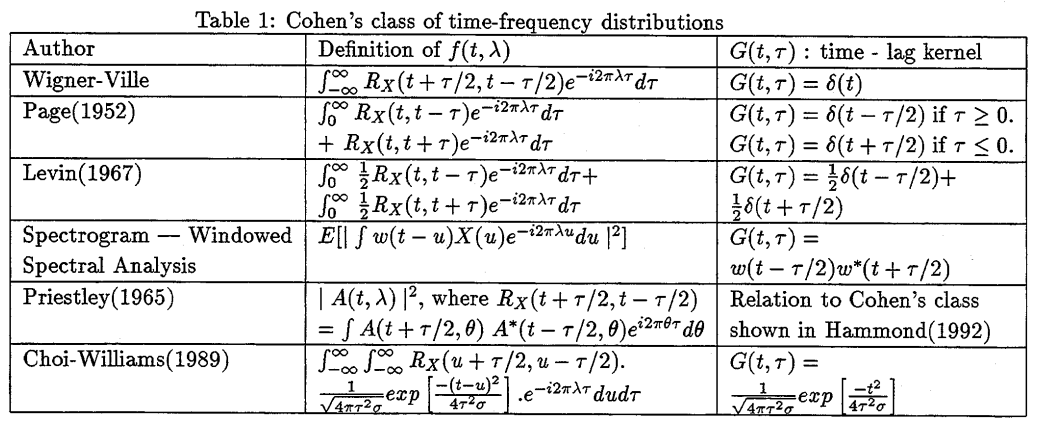
\includegraphics[width=0.9\textwidth]{tabla.png} 
%\end{figure}

%%%%%%%%%%%%%%%%%%%%%%%%%%%%%%%%%%%%%%%%%

%\subsection{Test Priestley-Subba Rao (PSR)}
%
%%(seccion en proceso de re-redaccion)
%
%A muy grosso modo, el test PSR estima localmente  el espectro evolutivo
% y revisa si estad\'isticamente
%cambia en el tiempo.
%
%Para ello, usa un estimador para la funci\'on de densidad espectral
%que es aproximadamente (asint\'oticamente) insesgado y cuya varianza est\'a
%determinada aproximadamente. La estimaci\'on se lleva a cabo en puntos en el tiempo y
%la frecuencia tales que en conjunto son aproximadamente no-correlacionados.
%Se aplica logaritmo para que la varianza de todos los estimadores sea aproximadamente
%la misma (el logaritmo ayuda a), amen que los errores conjuntos tengan una
%distribuci\'on cercana a una multinormal con correlaci\'on cero.
%Finalmente se aplica una prueba ANOVA de varianza conocida.

%%%%%%%%%%%%%%%%%%%%%%%%%%%%%%%%%%%%%%%%%%%%%%%%%%%%%%%%%%%%%%%%%%%%%%%%%%%%%%%%%%%%%%%%%%%%%%%%%%%

%\subsection{El espectro evolutivo}
%
%Consid\'erese un proceso estoc\'astico a tiempo continuo $\{X(t)\}$, tal que
%$E[X(t)]=0$ y $E\left[ X^{2}(t)\right] < \infty$ para todo $t$. Es decir que su media es constante
%y sus segundos momentos est\'an bien definidos, aunque 
%estos \'ultimos pueden cambiar con el tiempo.
%
%Por el momento se supondr\'a que acepta una representaci\'on de la forma
%
%\begin{equation*}
%X(t) = \int_{-\pi}^{\pi} A(t ; \omega) e^{i\omega t} \, d Z(\omega)
%\end{equation*}
%
%Con $\{ Z(\omega) \}$ una familia de procesos ortogonales\footnote{De nuevo, esto implica que
%$\Cov{dZ(\omega_1,dZ(\omega_2))} = \delta(\omega_1,\omega_1) d\omega$, una condici\'on m\'as
%d\'ebil que la independencia} tales que
%
%\begin{itemize}
%\item $E \left[\abso{ dZ(\omega)}^{2} \right] = d\omega$
%\item Para cada $t$ el m\'aximo de $A(t;\cdot)$ se encuentra en 0
%\end{itemize}
%
%Esta representaci\'on es an\'aloga a la representaci\'on de Cram\'er para un proceso
%estacionario, salvo que se permite que la funci\'on $A$ cambie con el tiempo.
%Siguiendo la analog\'ia, se define 
%el \textbf{espectro evolutivo} de $\{X(t)\}$, con respecto a la la familia
%$\mathcal{F} = \{ e^{i\omega t} A(t; \omega) \}$
% como
% 
%\begin{equation*}
%d F(\omega;t) = \lvert A(t;\omega) \lvert^{2} d\omega
%\end{equation*}
%
%Ahora bien, si se supone que $\{X(t)\}$ es estoc\'asticametne diferenciable, entonces
%se puede definir una \textbf{funci\'on de densidad espectral}
%
%\begin{equation*}
%f(t;\omega) = \lvert A(t;\omega) \lvert^{2}
%\end{equation*}
%
%Cabe destaca que si la funci\'on $A(t;\omega)$ fuera constante con respecto a $t$, se obtendr\'ia
%un proceso estacionario de orden dos tal cual fue descrito en la secci\'on anterior.

%%%%%%%%%%%%%%%%%%%%%%%%%%%%%%%%%%%%%%%%%%%%%%%%%%%%%%%%%%%%%%%%%%%%%%%%%%%%%%%%%%%%%%%%%%%%%%%%%%%

\subsection{El test PSR}

Esta t\'ecnica fue presentada por Priestley en 1965 \cite{Priestley69}; 
muy grosso modo, consiste en estimar localmente  el espectro
del proceso en cuesti\'on y revisa si se puede rechazar la hip\'otesis de que no
var\'ia en el tiempo.
%
%Para ello, usa un estimador para la funci\'on de densidad espectral
%que es aproximadamente (asint\'oticamente) insesgado y cuya varianza est\'a
%determinada aproximadamente. La estimaci\'on se lleva a cabo en puntos en el tiempo y
%la frecuencia tales que en conjunto son aproximadamente no-correlacionados.
%Se aplica logaritmo para que la varianza de todos los estimadores sea aproximadamente
%la misma (el logaritmo ayuda a), amen que los errores conjuntos tengan una
%distribuci\'on cercana a una multinormal con correlaci\'on cero.
%Finalmente se aplica una prueba ANOVA de varianza conocida.
%Muy a grosso modo, es un estimador de la
%funci\'on de densidad espectral con ciertas propiedades y que parte de la idea que un proceso
%no-estacionario puede verse localmente como un proceso lineal generalizado.
Muy a grosso modo, supone que localmente todo proceso estoc\'astico a tiempo continuo de varianza 
finita puede verse como un proceso lineal generalizado que es d\'ebilmente estacionario;
luego se pueden usar las ventanas espectrales y los filtros LIS sobre una porci\'on 
de tiempo ''peque\~na'' para estimar el espectro localmente.



%Como meta-nota, yo empec\'e a estudiar este tipo de estimadores porque es \textit{el qeu ven\'ia
%con el m\'etodo} ya que el test esta implementado en R; desde un punto de vista de difusi\'on,
%es una ventaja usar un m\'etodo implementado en un software gratuito y de c\'odigo abierto --y
%no una mera excusa para no explorar otros m\'etodos. En todo caso, he revisado varios otros test,
%pero de momento solo este ha arrojado suficientes resultados para llenar un informe.

%{Estimador de doble ventana (Priestley, 1965 \& 1966)}
Para construir el estimador se reuieren dos funciones, $g$ y $w_T$, que servir\'an como ventanas
para extraer informaci\'on local de los datos. Debido a que sus propiedades tienen una interpretaci\'on
f\'isica desde la teor\'ia de circuitos, absorben su terminolog\'ia

\textit{
nota al pie: deberia incluir una motivacion de estos nombres,
que en parte tiene relevancia en la interpretacion. Los 
Linear Invariant Systems (LIS) suponen dependencia lineal
--constante-- respecto a todos los tiempos anteriores; 
a tiempo continuo son equivalentes a una ecuacion diferencial ordinaria lineal,
y a su vez a modelos AR. Un modelo fisico para ello son los circuitos RC, que
fueron usables en radios, y para los cuales las palabras 'filtro' y 'frecuencia'
tienen una interpretacion clara. Esta terminologia de circuitos electricos tiene sentido
para mi ya que todos los modelos de neuronas y poblaciones de neuronas que he visto hasta ahora,
por ejemplo de Ermentrout (falta citar), {Clark98,Priestley81}, PARTEN de considerar
circuitos equivalentes a los componentes neuronales, lo cual me hace pensar que es buena idea
mantener esta vision conjunta.
}

Primeramente se toma una funci\'on $g(u)$ normalizada, que en conjunto a su
transformada inversa de Fourier\footnote{Esta funci\'on 
$\Gamma(u) = \int_{-\infty}^{\infty} g(u) e^{i u \omega} du$
es referida como
\textbf{frequency-response function}, nombre tiene un poco de encanto cuando
$g$ adopta ciertas formas particulares (senos y cosenos).} 
$\Gamma$ tiene las siguientes propiedades

\begin{equation*}
2\pi \int_{-\infty}^{\infty} \lvert g(u) \lvert^{2} du 
= 
\int_{-\infty}^{\infty} \lvert \Gamma(\omega) \lvert^{2} d\omega
= 1
\end{equation*}


A partir de $g$ y $\Gamma$ se define el filtro $U$ como una convoluci\'on
con las realizaciones del proceso

\begin{equation*}
U(t,\omega) = \int_{t-T}^{t} g(u) X({t-u}) e^{i \omega (t-u)} du
\end{equation*}

Un ejemplo que est\'a en el libro de Priestley es tomar funciones del tipo

\begin{equation*}
g_h(u) = 
\begin{cases}
{1 \big{/} 2\sqrt{\pi h}} & \text{ , } \abso{u} \leq h
\\
0 & \text{ , } \abso{u} > 0
\end{cases}
\end{equation*}

Su correspondiente funci\'on de respuesta de frecuencia es complicada [me falta 
escribirla]. Es referida como la \textbf{ventana de Bartlett} y
est\'a totalmente caracterizada la siguiente propiedad

\begin{equation*}
\abso{\Gamma_h(\omega)}^{2} = \frac{1}{\pi h} \left( \frac{\text{sen} (h \omega)}{\omega} \right)^{2}
\end{equation*}

Cabe mencionar que puede entenderse al par $g$ y $\Gamma$ como ventanas en el tiempo
y las frecuencias para la serie.

---

Ahora bien, se toma una funci\'on $W_\tau$ que cubre el papel de ventana de retrasos,
con su respectiva ventana espectrasl $w_\tau$; se piden las siguientes propiedades

\begin{itemize}
\item $w_{\tau}(t) \geq 0$ para cualesquiera $t$, $\tau$
\item $w_{\tau}(t) \rightarrow 0$ cuando $\lvert t \lvert \rightarrow \infty$, para todo $\tau$
\item $\displaystyle \int_{-\infty}^{\infty} w_{\tau}(t) dt = 1$ para todo $\tau$
\item $\displaystyle \int_{-\infty}^{\infty} \left( w_{\tau}(t) \right)^{2} dt < \infty$ para todo $\tau$
\item $\exists C$ tal que  
$\displaystyle \lim_{\tau\rightarrow\infty} \tau \int_{-\infty}^{t} \abso{ W_{\tau}(\lambda) }^{2} d\lambda = C$
\end{itemize}
%[T est\'a relacionado con el 'tiempo 0', pero para
%tiempos de muestreo grandes se puede reemplazar por $-\infty$ EXCEPTO cerca del inicio y el final dle muestreo]
%$$\lim_{\tau\rightarrow\infty} \left[ \tau \int_{t-T}^{t} \lvert W_{\tau}(\lambda) \lvert^{2} d\lambda \right] = C$$
%Ahora, si se define 
%$\displaystyle W_{T'}(\lambda) = \int_{-\infty}^{\infty} e^{-i\lambda t}w_{T'}(t) dt $
%[posteriormente annadire mas detalles sobre el papel que juega el par $w_\tau$, $W_\tau$]

%Como ejemplo, se puede tomar la siguiente funci\'on llamada \textbf{ventana de Daniell}

%\begin{equation*}
%W_\tau (t) = 
%\begin{cases}
%{1 \big{/} \tau} & \text{ , } -\nicefrac{1}{2} \tau \leq t \leq \nicefrac{1}{2} \tau
%\\
%0 & \text{ , otro caso}
%\end{cases}
%\end{equation*}
%
%La cual se puede demostrar [tengo en algun lado esa demostracion]

Por ejemplo, se puede calcular que para la ventana de Daniell

$$\lim_{\tau\rightarrow\infty} \tau \int_{t-T}^{t} \lvert W_{\tau}(\lambda) \lvert^{2} d\lambda = 2\pi$$

-----

Se define el estimador para $f_t$, con $0 \leq t \leq T$
\begin{equation*}
\widehat{f_t}(\omega) = \int_{t-T}^{t} w_{T'}(u) \lvert U(t-u,\omega) \lvert^{2} du
\end{equation*}

Fue demostrado por Priestley (1965, falta citar) que 

[aqui van las expresiones para el valor esperado y la varianza de $\widehat{f_t}$, me falta
escribirlas]

Pero, bajo varios supuesto adicionales [que me falta trascribir] se puede aproximar

\begin{equation*}
E\left[ \widehat{f_t}(\omega) \right] \sim f_t(\omega)
\end{equation*}

\begin{equation*}
\Var{\widehat{f_t}(\omega)} 
\sim 
\frac{C}{\tau} \left(f_t(\omega)\right)^{2} \int_{-\infty}^{\infty} \abso{\Gamma(\theta)}^{4} d\theta
\end{equation*}

Se advierte claramente que $\widehat{f_t}$ es unnestimados aproximadamente insesgado.
Para las ventanas de Bartlett y Daniell usadas como ejemplo, se tiene

\begin{equation*}
\Var{\widehat{f_t}} 
\sim 
\frac{4h}{3\tau} \left(f_t(\omega)\right)^{2}
\end{equation*}

Cabe mencionar que hay una expresi\'on expl\'icita para la covarianza de $\widehat{f_t}$
en para diferentes puntos en el tiempo y las frecuencias. Lamentablemente,
aun me falta escribirlas, son complicadas, y se describen situaciones bajo las
cuales estas covarianzas son negligibles; cabe destacar que TODAS las condiciones 
que se usan para aproximar son b\'asicamente las mismas, y dependen de que la distancia
entre los tiempos y las frecuencias sean tan grandes como sea posible.

------------

El \'ultimo ingrediente del test PSR es una transformaci\'on logar\'itmica
para regular la varianza, y quiza para cortar los bordes de las aproxiamciones.
Se define $Y_{i,j} = \log \left( \widehat{f_{t_i}}(\omega_j) \right)$, con las siguientes propiedades

\begin{equation*}
E\left[ Y_{i,j} \right] \thicksim \log \left( f_{t_i}(\omega_j) \right)
\hspace{4em}
\text{Var}\left( {Y\left(t,\omega\right)}\right) \thicksim \sigma^{2}
\end{equation*}

Luego as\'i, puede escribirse aproximadamente que

$$Y_{i,j} = \log \left( f_{t_i}(\omega_j) \right) + \varepsilon_{i,j}$$

donde $\varepsilon_{i,j}$ va iid tales que

$
E\left[ \varepsilon_{i,j} \right] = 0
\hspace{4em}
\text{Var}\left( \varepsilon_{i,j} \right) \sigma^{2}
$

Priestley cita que con esta informaci\'on incluso se puede considerar que los $\varepsilon_{i,j}$
siguen una distribuci\'on normal cada uno; Nason (2015, falta citar) comenta que
este supuesto no tiene por que cumplirse, y que es una popsible fuente de falsos positivos
para el test. Yo he hecho pruebas de normalidad a los datos, que incluire como anexos
mas tarde.

El test PSR \textit{per se} son tres test ANOVA --en su versi\'on en la que la varianza es conocida--
sobre si los $\varepsilon_{i,j}$ son estad\'isticamente negligibles en total, sobre el tiempo y sobre
las frecuencias. Para el fin de estudiar la estacionariedad, basta con que sean estad\'iticamente
no-negligibles sobre el tiempo.

%[Por supuesto que los otros dos test tienen interpretacion: la negigibilidad total da informacion
%sobre las marginales, y si estas pueden ser estimadas adecuadamente usando el estimador, si se
%combina con negativo para no-estacionariedad es \textbf{efectivamente positivo} para estacionariedad
%y toma una forma muy particular (proceso uniformemente modulado). Si sobre las frecuencias resulta
%significativo (no-negligible) da informacion sobre la 'aeatoridad total' del proceso.
%De tener tiempo, lo incluire como anexo, ya que ninguna de estas caracteristicas es estudiada :( ]

%Lo detalles de la implementaci\'on en R estar\'an en la secci\'on de resultados.

%%%%%%%%%%%%%%%%%%%%%%%%%%%%%%%%%%%%%%%%%%%%%%%%%%%%%%%%%%%%%%%%%%%%%%%%%%%%%%%%%%%%%%%%%%%%%%%%%%%
%%%%%%%%%%%%%%%%%%%%%%%%%%%%%%%%%%%%%%%%%%%%%%%%%%%%%%%%%%%%%%%%%%%%%%%%%%%%%%%%%%%%%%%%%%%%%%%%%%%